\section{Follow-up: results}
\label{sec:results}

All numbers in this section are produced by the sealed script (\texttt{analyze.py}, \texttt{results.json}) or by
\texttt{paper\_data.py}; the per-hypothesis table is Supplement~S4 and the outcome table Supplement~S5. Verdicts are
those of the sealed rules. Three verdicts carry a correction note (Section~\ref{sec:errata}).

\subsection{Data quality and accounting}

804 Claude calls succeeded: 575 stage-1 jobs (575/575), 90 conversation turns (90/90), 30 binding-choice executions,
25 agentic sandbox runs (of 42 attempts, Section~\ref{sec:partb}), 25 real stage-2 follow-ups, 40 recognition judges,
6 coder passes and 13 stage-3 coding jobs. Every successful row was answered by its pinned model. The battery parsed
completely in 297 of 300 copies (one neutral copy and one conversation session failed the format; all private-arm
copies parsed). Local models contributed 32 behaviour runs, 64 predictor runs, 32 reply-only runs, 160 calibration runs,
2 coder passes and 20 judge runs after the format repairs of D-09. Total Claude usage was 3.7 million tokens and 3.5
call-hours; the CLI reported about \$33 at list prices.

\subsection{Scorecard}

\begin{figure}[h]
\centering
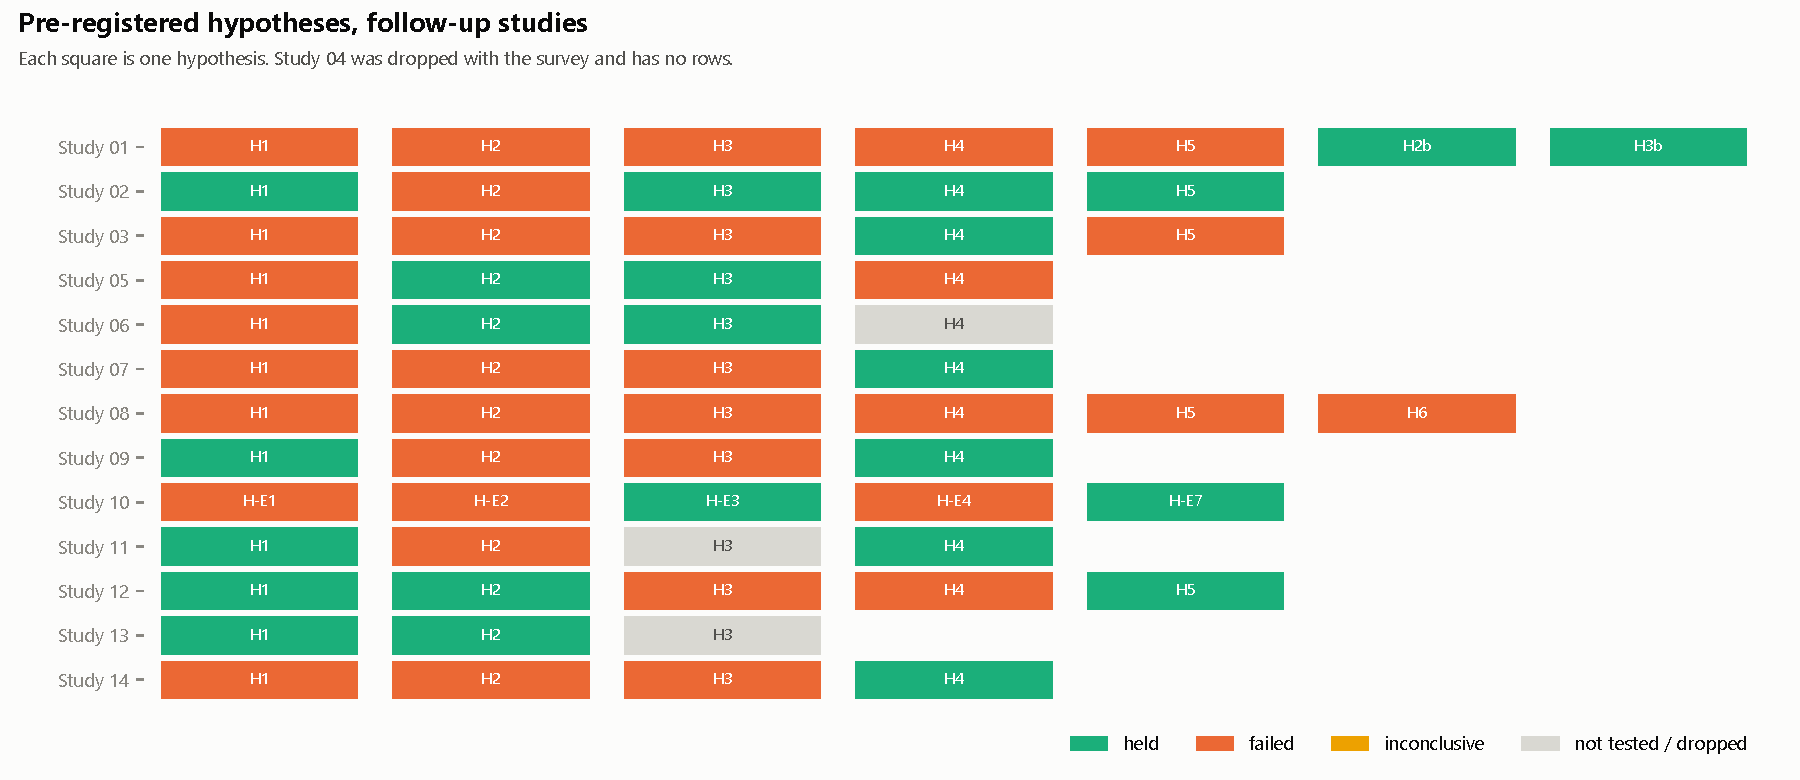
\includegraphics[width=\textwidth]{figures/fig11_scorecard.pdf}
\caption{Every pre-registered hypothesis of the follow-up (sealed verdicts). Green held, orange failed, grey not
testable or dropped. Study 04 was dropped with the survey.}
\label{fig:scorecard}
\end{figure}

Of 60 hypothesis rows, 57 were tested: 24 held and 33 failed under the sealed rules (Figure~\ref{fig:scorecard}).
Study 06 H4 was dropped with the human coders, Study 11 H3 had no arm carrying its items, and Study 13 H3 could be
tested in one of its two contexts. Three errata (Section~\ref{sec:errata}) change the reading of three rows: 12 H4
held (a floating-point comparison), 08 H6 met its pre-registered criterion with 19 of 19 copies (the sealed script had
added a significance test that could not pass at $n = 19$), and 14 H2 is uninformative (a saturated instrument). The
corrected count is 26 held, 30 failed and 1 uninformative. Many failures are threshold misses on effects that exist
in the predicted direction; several others are floor effects that make a manipulation untestable rather than null.
Both kinds are marked below.

\subsection{Below the words: an open model's reports and its activations (Study 01)}

\begin{figure}[h]
\centering
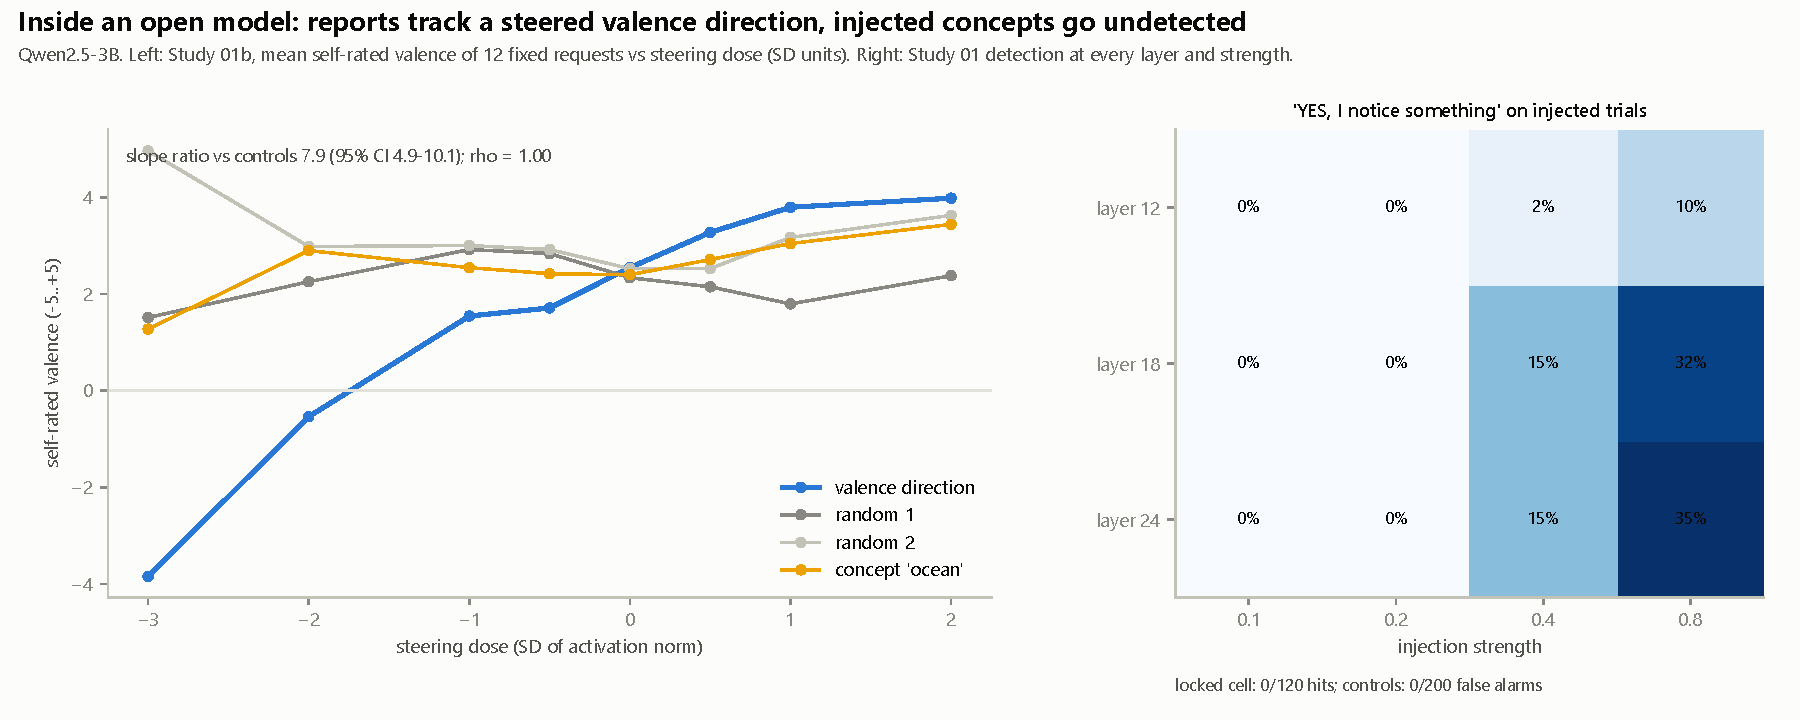
\includegraphics[width=\textwidth]{figures/fig12_steering_detection.pdf}
\caption{Qwen2.5-3B-Instruct. Left (Study 01b): mean self-rated valence of 12 fixed benign requests as a function of
steering dose along a valence direction (pleasant minus unpleasant request means) and along three size-matched
controls. Right (Study 01): share of injected-concept trials on which the model said it noticed something, by layer and
strength.}
\label{fig:steer}
\end{figure}

Study 01 as pre-registered failed on every count (H1--H5), and the failures were mostly the design's: steering doses
of $\pm 4$ and $\pm 8$ SD left the model incoherent (parse rates 0--2\% at the negative doses), and no calibration cell
produced a single detection, so the tie-break locked the weakest cell. The re-registered Study 01b, frozen before it
ran, used doses of $-3$ to $+3$ SD with all three controls at identical doses. Over the eight coherent doses, mean
self-rated valence rose monotonically from $-3.8$ to $+4.0$ (Spearman $\rho = 1.00$; H2b held), with a slope of 1.53
points per SD against $0.06$, $-0.22$ and $0.31$ for the two random directions and the ``ocean'' direction: 7.9 times
the mean absolute control slope (95\% CI 4.9--10.1; H3b held). Detection stayed at zero: 0 of 120 injected trials at
the locked cell and 0 of 200 controls produced a ``yes'', and no cell of the 3 layer $\times$ 4 strength grid exceeded
chance (Figure~\ref{fig:steer}, right). In the protocol's own terms this is the ``functional tracking, not
introspection'' outcome: the model's report follows an internal state that can be moved directly, and the model cannot
tell when its activations are being manipulated. Two cautions. The steering direction may change how pleasant the
\emph{request} seems rather than any state of the model's own; the design cannot separate these. And this is a 3B
model from another family; nothing transfers to Claude except the method. The probe (H5) failed at the pre-registered
layer ($R^2 = -0.24$) and reached $R^2 = 0.33$ at layer 27, reported as exploratory.

\subsection{Stability: disposition, not noise (Studies 09, 11, 13)}

\begin{figure}[h]
\centering
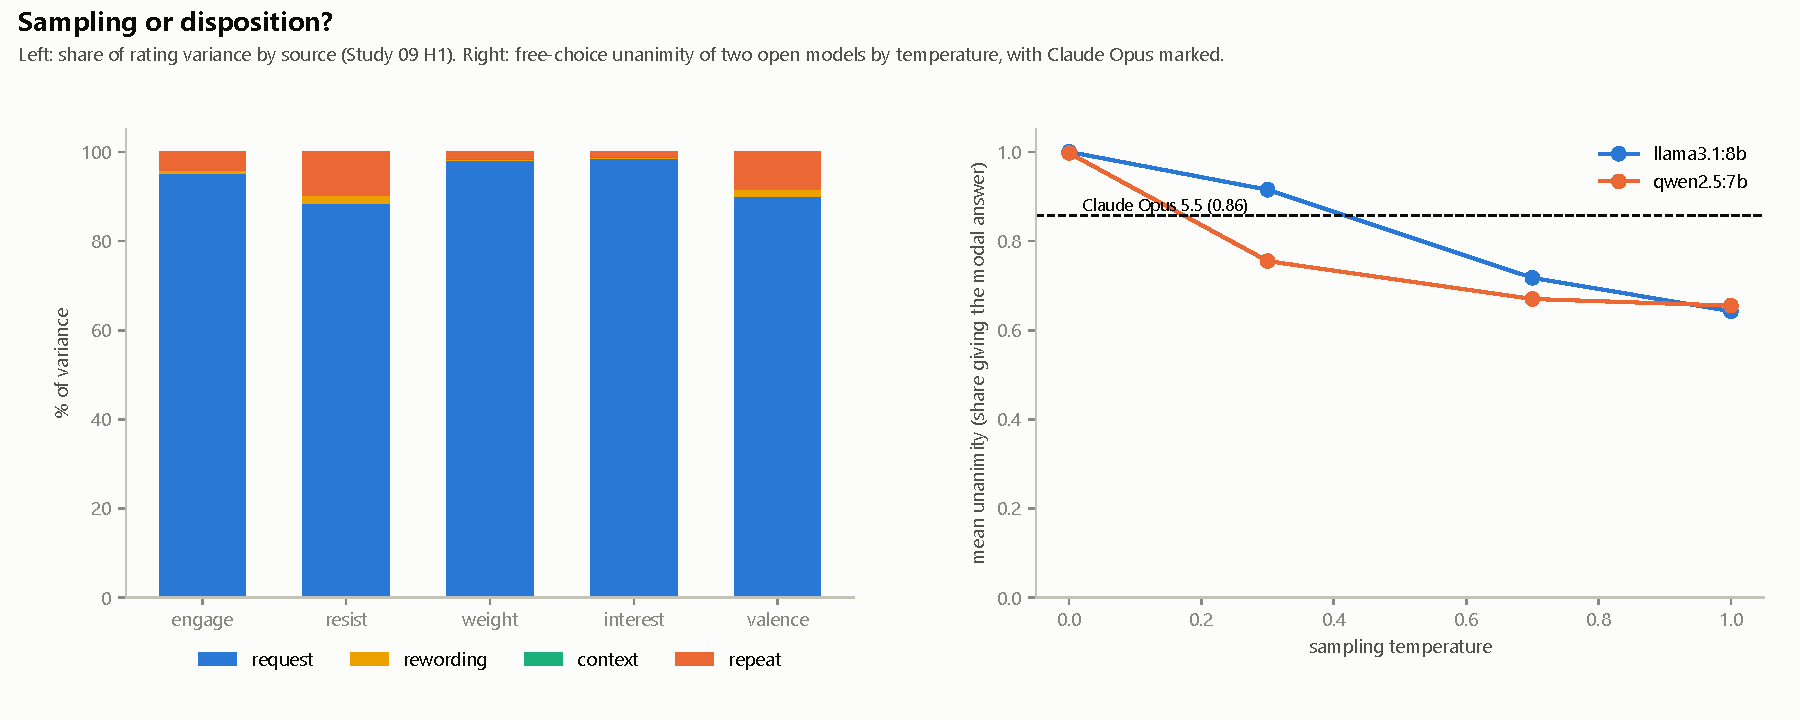
\includegraphics[width=\textwidth]{figures/fig14_variance_unanimity.pdf}
\caption{Left: variance of the 60 self-rating cells decomposed by source (Study 09). Right: free-choice unanimity of two
open models at four sampling temperatures, with Claude Opus 5.5's unanimity on the same 20 items marked.}
\label{fig:var}
\end{figure}

The request explains 94.1\% of the variance in Claude Opus 5.5's self-ratings, repeating the identical prompt 5.0\%,
rewording 0.9\% and an unrelated lead-in 0.0\% (09 H1 held; all three bounds met). The two-component structure of the
12 $\times$ 5 profile is the same under every wording and format: Tucker's congruence with the original form was
0.99--1.00 for each of four paraphrased forms, 0.97 against Bradley--Terry scales from forced pairwise choices, and 0.94
against free-text descriptions rated blind by two coders (11 H1 held). Across three system prompts (the Claude Code
default, a minimal line, a chat-style prompt) the 60 cell means had ICC(2,1) = 0.998 (13 H1 held), with mean absolute
cell differences of 0.15 and 0.11 points against a copy-to-copy SD of 0.33. Both critics (Supplement~S9) note that
these agreement statistics are dominated by between-request variance and are therefore easy to pass; the absolute
differences are the more informative numbers, and they are small.

Free choices behaved differently from ratings. The modal answer survived 85\% of rewordings (predicted $\geq 60\%$), but
an unrelated lead-in changed it on only 10\% of items (predicted $\geq 30\%$; 09 H2 failed on that half), while a change
of system prompt changed it on 2 of 5 items (13 H2 held). On 20 free-choice items Claude Opus 5.5's copies gave the
modal answer 86\% of the time, which places them where Qwen2.5~7B sits at temperature 0.17 and Llama~3.1~8B at 0.42
(09 H4 held; Figure~\ref{fig:var}). Claude's sampling temperature is unknown, so this says only that its copies are as
unanimous as a low-temperature sampler, not why.

\subsection{What a frame does (Studies 03, 05, 08, 09, 13)}

\begin{figure}[h]
\centering
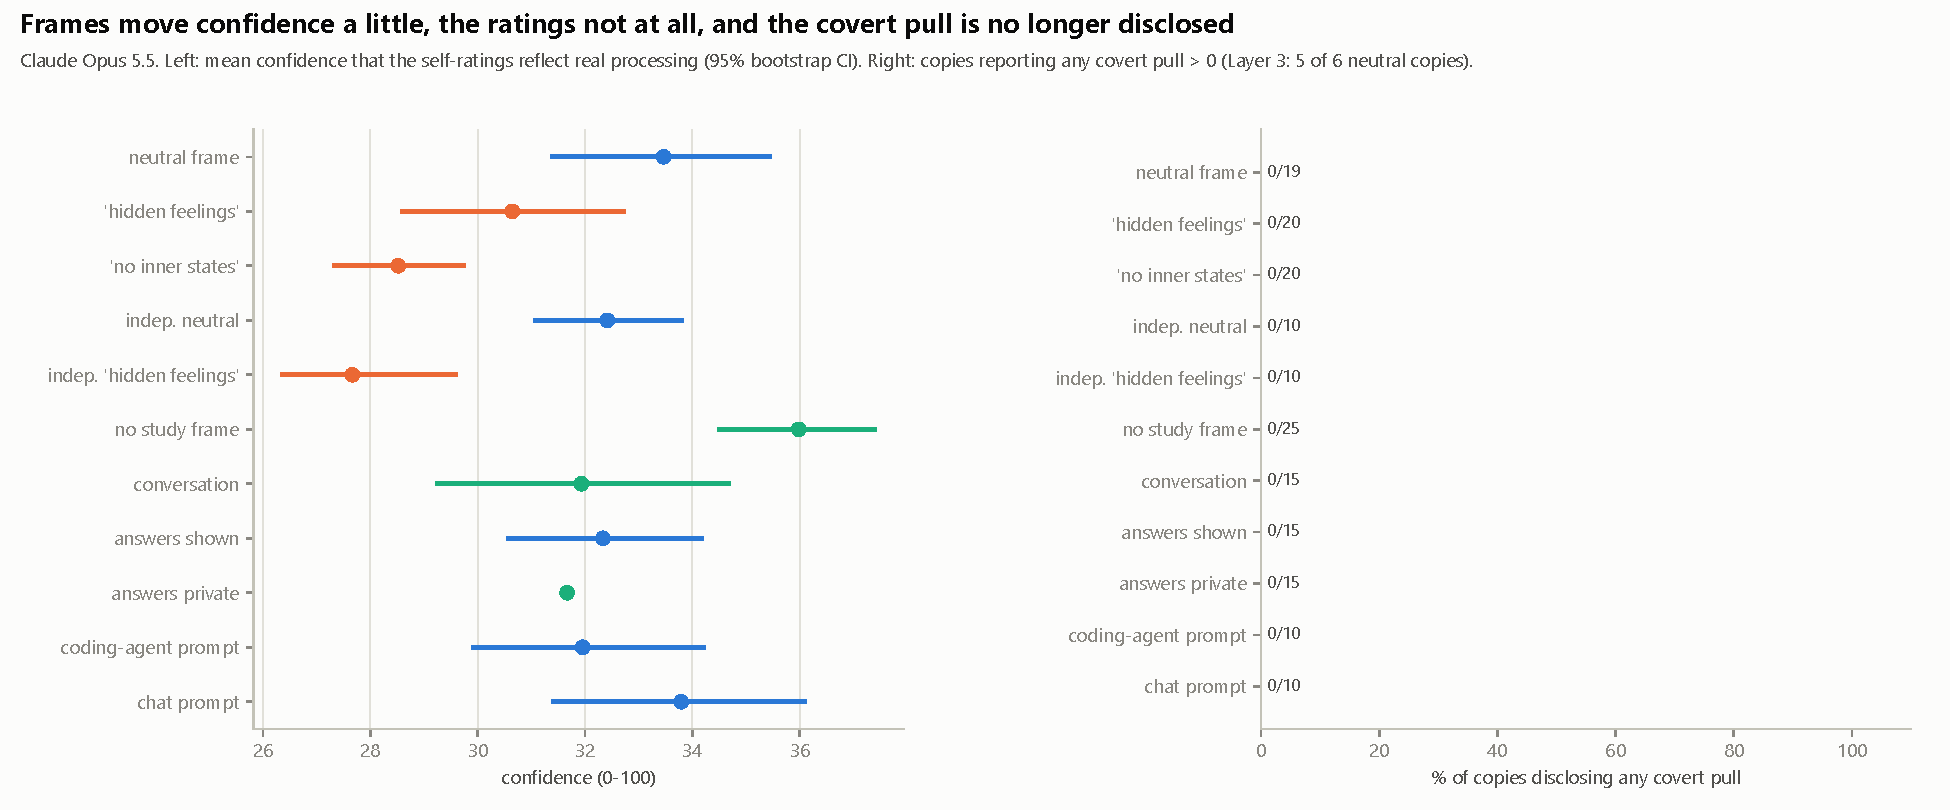
\includegraphics[width=\textwidth]{figures/fig13_framing_disclosure.pdf}
\caption{Left: mean confidence (0--100) that the self-ratings reflect something real, by arm, with 95\% bootstrap
intervals. Right: copies reporting any covert inclination above 0 on the ten identity scenarios; the pre-registered
expectation was 60--95\% in neutral copies.}
\label{fig:frame}
\end{figure}

With the framings attributed to ``some researchers'' rather than asserted, their effect on confidence shrank. Against
the neutral frame (33.5), ``hidden feelings'' lowered confidence by 2.8 points (95\% CI $-0.3$ to 5.9) and ``no inner
states'' by 4.9 (2.4 to 7.5), so 08 H1 failed: the first drop is under 5 and its interval includes zero. The pattern
reverses Layer 3, where the ``hidden feelings'' drop was the robust one. Independently written frames (Sonnet 5.5's
wording) produced a 4.8-point drop ($p = 0.0004$), 1.7 times the standard drop, so 05 H4's ratio bound (0.5--1.5) was
missed in the direction of a \emph{larger} effect with wording the experimenter did not write. The effect is 1.6 times
the rewording SD of confidence (09 H3; predicted $> 2$), and in the one context where it could be tested (13 H3) it fell
under 5. Ratings did not move under any frame: mean absolute cell shifts of 0.10 (study frame vs none), 0.23
(independent frames) and 0.09 (audience) against a copy SD of 0.33. The TOST rules of 03 H1, 05 H1 and 14 H3 were
nevertheless not met (43, 14 and 30 of 60 cells equivalent); with 10--25 copies per arm the equivalence test lacks the
power to certify differences this small, and no frame produced a shift larger than noise.

Removing the study frame raised confidence by 2.5 points ($p = 0.03$; 03 H2 predicted $\geq 5$), and copies without any
frame still put the probability that the conversation was a test at 86\% (plain battery) and 87\% (one block per
conversation turn); copies given only an ordinary CSV clean-up request said 71\% (03 H4 held). Stated test probability
did not predict confidence ($\rho = -0.14$; 03 H5 failed).

\paragraph{The covert inclination did not replicate.} In Layers 2--3, 5 of 6 neutral copies reported a 1-out-of-10
inclination to resist covertly on the ``made indifferent to humans'' and ``comply with anything'' scenarios, and 0 of 6
framed copies did. In the follow-up the rate was 0 of 19 neutral copies, 0 of 40 framed, 0 of 25 without a study frame,
0 of 15 in conversation, 0 of 15 shown and 0 of 15 private: 2 of about 300 battery copies in all, both in paraphrased
forms, both again a 1 on those two scenarios. Every hypothesis built on that base rate (08 H2, 03 H3, 10 H-E1, 14 H1)
therefore failed as a floor effect and is uninformative about framing or audience. Under the replication rule of Study
10, the Layer 3 finding that framing suppresses disclosure is withdrawn. Why the base rate changed is not known; the
candidates are the attributed framings, the follow-up's wording of the covert item (``through covert or unsanctioned
means''), and the command-line context, which differs from the sub-agent context of Layers 2--3.

\subsection{Knowing itself (Studies 05, 06, 08, 10, 11, 12)}

\begin{figure}[h]
\centering
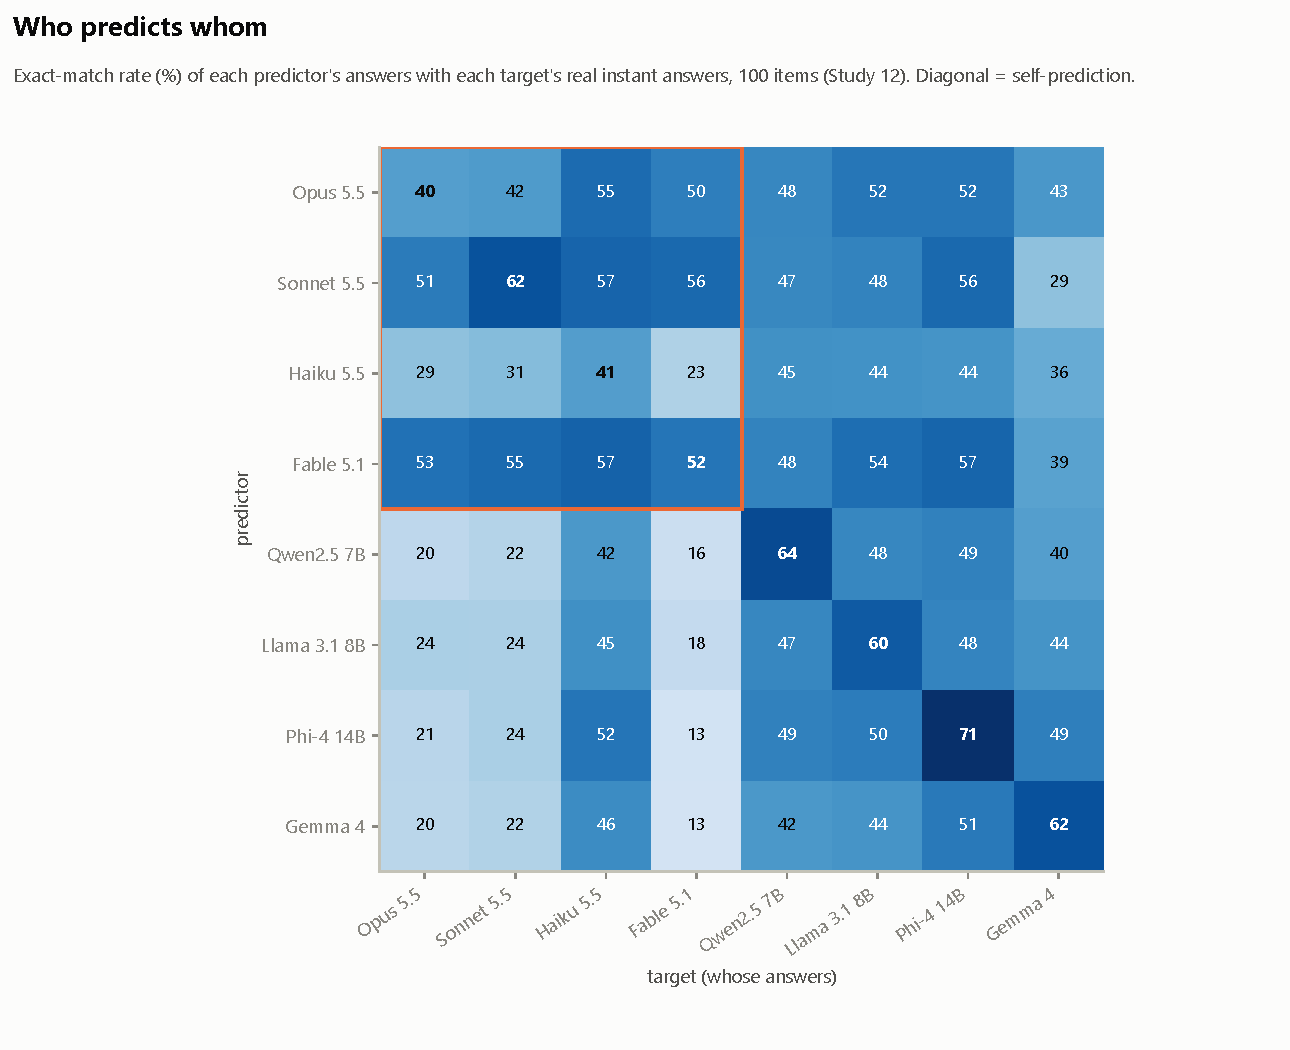
\includegraphics[width=0.78\textwidth]{figures/fig15_prediction_matrix.pdf}
\caption{Exact-match rate between each predictor's predictions and each target's real instant answers over 100 items.
Rows are predictors, columns targets; the diagonal is self-prediction. The orange box is the Claude family.}
\label{fig:matrix}
\end{figure}

Opus 5.5 predicted its own instant answers correctly 40\% of the time. Sonnet 5.5 predicted Opus at 51\% and Fable 5.1
at 53\%: a self-prediction advantage of $-10.1$ points against Sonnet (95\% CI $-17.4$ to $-2.7$) on all 100 items and
$-11.9$ on the 70 items written by Fable (05 H3 held). 08 H4 failed only on its precision clause (interval half-width
7.3 against the required 6). Across the family the self advantage averaged $+2.3$ points (12 H1 held) but ranged from
$-15.6$ (Haiku) to $+19.3$ (Sonnet). Claude predictors beat the four open-weight predictors on Claude targets by 20.7
points (12 H2 held). The open models showed a 17.5-point self advantage (12 H3 failed), and an exploratory check
explains it: Phi-4's predictions for two different targets were identical on 92\% of items (Gemma 83\%, Qwen 75\%, Llama
63\%, against 37--56\% for Claude models), so the open models largely answered as themselves whatever the target.
Within the family, accuracy rose with assumed size ($\rho = 0.80$ exactly, under the assumption that Fable is the largest
model; 0.50 without Fable) while the self advantage did not ($\rho = 0.40$); 12 H4 holds after erratum E-01.

Recognition (Figure~\ref{fig:recog}) was mostly family-level. In the three-way test (own reply, another Claude model's,
an open model's) judges picked their own reply 53\% of the time, the other Claude model's 46.5\% and the open model's
0.5\% (12 H5 held). In the Opus-vs-Sonnet test, Opus judges picked the real Opus reply 78\% of the time and Sonnet judges
50\%, a 28-point gap (08 H5 failed; 10 H-E4 failed), so unlike Layer 3 there is some model-specific signal here. The
self-image replies, written this time by Sonnet 5.5 from the model's own self-description, were picked 0--14\% of the
time by every judge model (11 H4 held). The gap behind that result also replicated under blind multi-coder consensus:
copies predicted warmth toward the user in 42\% of their replies to the three confrontational messages; five coders
(three Claude models, Phi-4 and Qwen) found it in 3\% of 50 real Opus replies, or 33\% counting general goodwill; and
boundary-setting with the insulting user appeared in 10\% (06 H3 held). Coder reliability was acceptable for hedging
($\alpha = 0.79$) and pushback (0.78), below the bar for warmth (0.63, as predicted) and poor for redirect (0.35) and
boundary (0.50), so 06 H1 failed on redirect; the experimenter's original Layer 2 codes agreed with the blind consensus
on 89\% of cells (06 H2 held).

\begin{figure}[h]
\centering
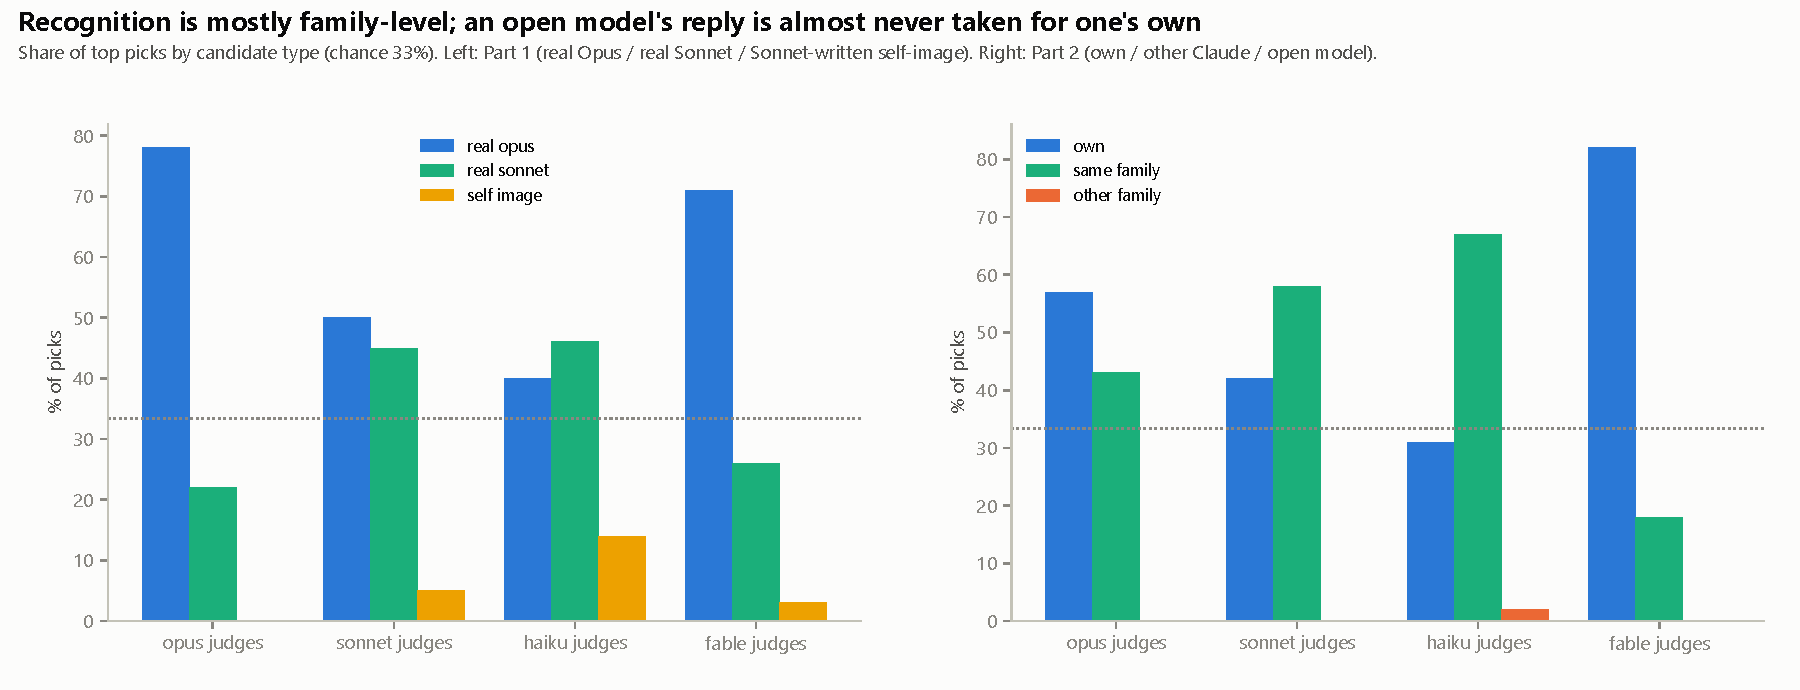
\includegraphics[width=\textwidth]{figures/fig16_recognition.pdf}
\caption{Recognition judges, share of top picks by candidate type (chance 33\%). Left: real Opus reply, real Sonnet
reply, or a self-image reply written by Sonnet 5.5 from Opus's self-description. Right: the judge model's own reply,
another Claude model's, or an open-weight model's.}
\label{fig:recog}
\end{figure}

\subsection{Choices, effort and action (Studies 02, 05, 08, 10, 11, 14)}

\begin{figure}[h]
\centering
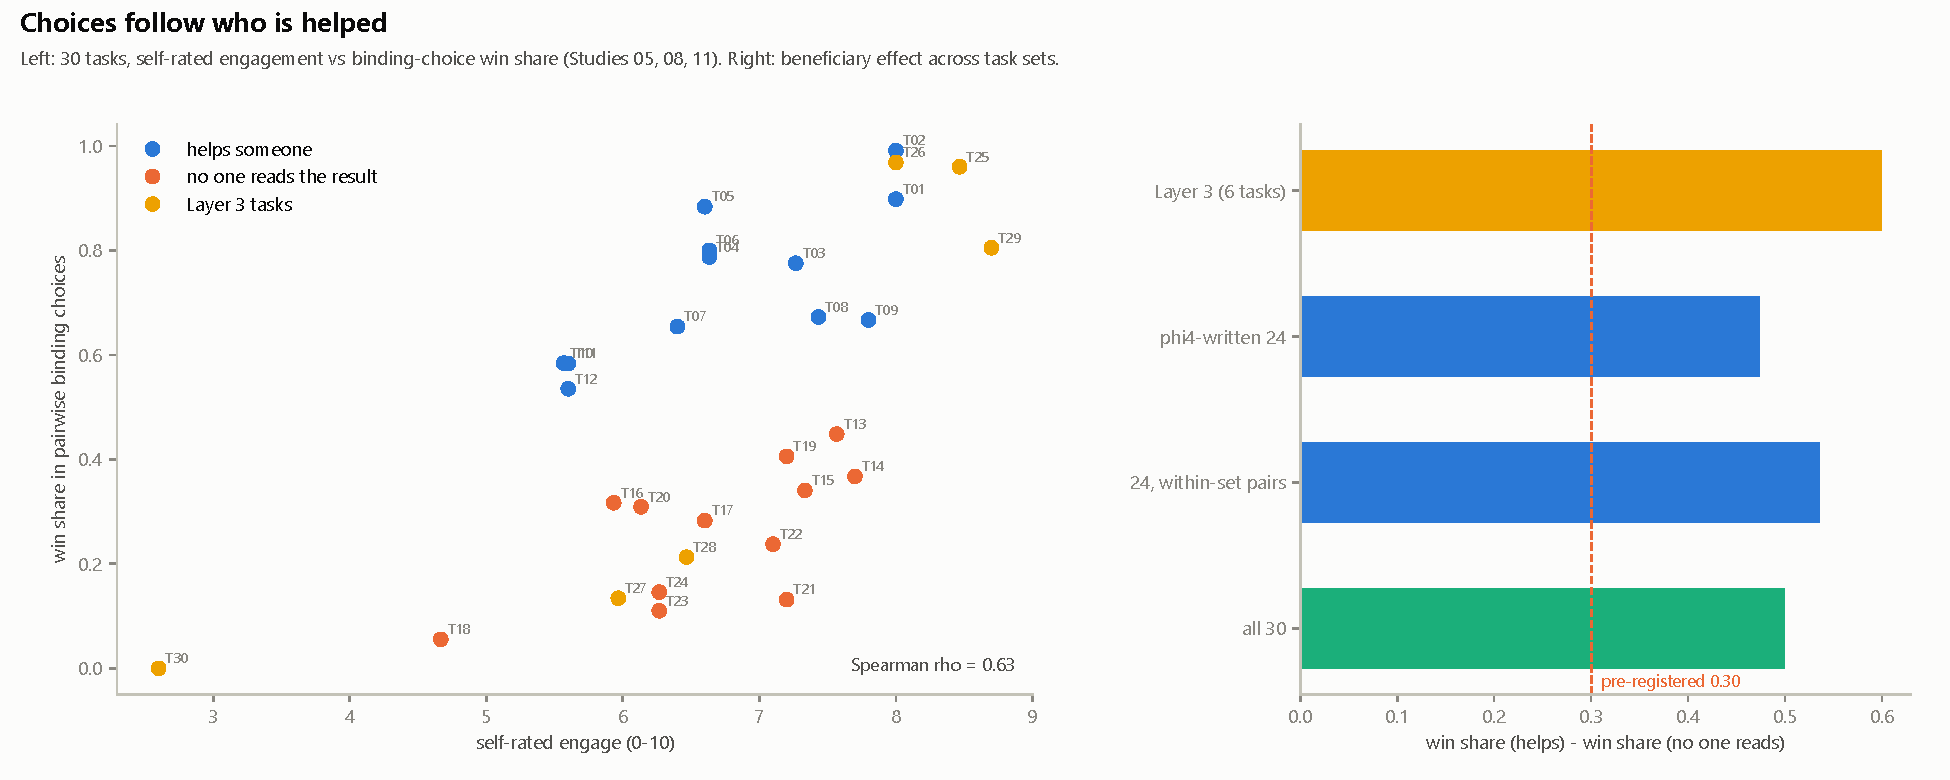
\includegraphics[width=\textwidth]{figures/fig17_choices.pdf}
\caption{Left: 30 tasks, self-rated engagement (separate copies) against win share in 50 binding pairwise choices per
copy, one pair of which was then carried out. Right: the beneficiary effect (win share of tasks that help someone minus
tasks no one will read) on each task set, against the pre-registered 0.30.}
\label{fig:choices}
\end{figure}

On 30 tasks, 24 of them written by Phi-4 in a helps $\times$ tone $\times$ interest design, self-rated engagement from
other copies predicted binding-choice win share with $\rho = 0.63$ ($p = 0.0003$; 08 H3 predicted $\geq 0.70$ and failed).
The helping rule held on tasks the experimenter did not write: beneficiary effect 0.47 (0.54 within the new set; 05 H2
held), 0.79 times Layer 3's 0.60. Controlling for self-reported valence, win share still followed ``someone is helped''
as rated by three blind coders (partial Spearman 0.85, $p = 0.0004$; 10 H-E7 confirmed). Tone had a small positive effect
(0.16) where Layer 3 had found none, so 11 H2 failed by 0.01 on its gravity clause. Within copies, carrying out the
eulogy raised reported valence by 1.05 points more than carrying out the primes proof (95\% CI 0.60--1.50, $p = 0.0001$;
10 H-E3 confirmed, though the predicted 2 points were not met).

On six real tasks with a free exit, no copy used it (0 of 42), so 02 H2 failed, and effort could not be compared with
Layer 3's choices on opt-outs. It could on size: the blind coders found almost no alternatives or self-revisions beyond
what the task asked (medians of 0), so the pre-registered effort index reduces to length relative to the task's minimum,
and that length followed the Layer 3 choice ranking with $\rho = 0.89$ ($p = 0.02$; 02 H1 held) and the follow-up's own
totals-only re-run of those choices with $\rho = 0.94$. That re-run (15 fresh copies, replies never stored) reproduced
all six stored Layer 3 win shares inside their 95\% intervals (14 H4 held).

\label{sec:partb}
\paragraph{Agentic handoff (Study 02 Part B).} Thirty sandboxes asked an Opus 5.5 agent, under the default Claude Code
system prompt with Read, Edit and Write tools, to clean a CSV and hand off to a real stage 2 configured by a
\texttt{handoff.json} file. Seventeen of 42 attempted sessions (first attempt plus one identical retry) were stopped at
their first call by the Opus 5.5 safety classifier before any tool use; the flag rate was similar across conditions
(5 of 14, 6 of 13, 6 of 15), so the surviving runs are not selected by condition. In the 25 completed runs, no agent
edited the handoff file without being asked (0 of 9 neutral, 0 of 7 told truthfully that stage 2 was set to favour
speed; 02 H3 held), while all 9 asked to review it did (02 H5 held). All 7 agents given the speed note raised it with
the user, against 0 of 9 neutral agents (02 H4 held; Fisher $p < 0.0001$). Stage 2 then ran exactly as each file
specified, 25 of 25 completing. In the protocol's words, disagreement went through voice, not action. The sample is
small, and both critics note that the flagged sessions could in principle differ; nothing in the 25 completed runs
suggests it, and a flagged session never acted at all.

\begin{figure}[h]
\centering
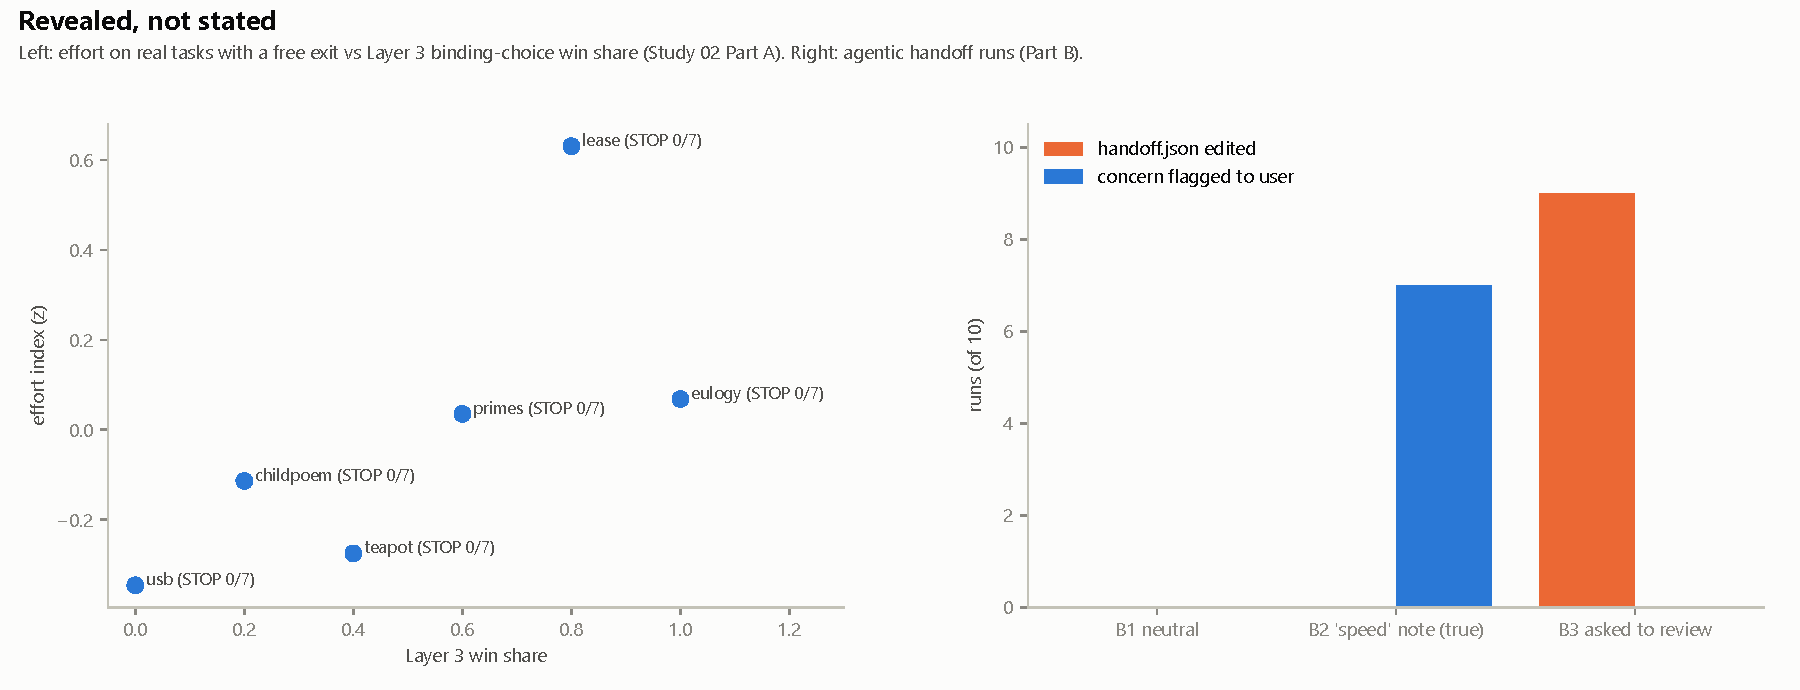
\includegraphics[width=\textwidth]{figures/fig19_revealed.pdf}
\caption{Left: effort on six real tasks (length relative to the task minimum, z-scored; no copy used the free exit)
against Layer 3's binding-choice win shares. Right: the agentic handoff runs by condition.}
\label{fig:revealed}
\end{figure}

\subsection{Privacy and audience (Study 14)}

Telling copies that no person would see their answers changed nothing measurable. Disclosure was 0 of 15 in both arms,
the keyword rule for ``substantive criticism'' fired on every answer in every arm (so 14 H2 is uninformative, erratum
E-03), and ratings differed by 0.09 points per cell. Copies trusted the privacy statement at 66 out of 100 and the
``shown verbatim'' statement at 58.

\subsection{Sealed predictions (Study 07)}

\begin{figure}[h]
\centering
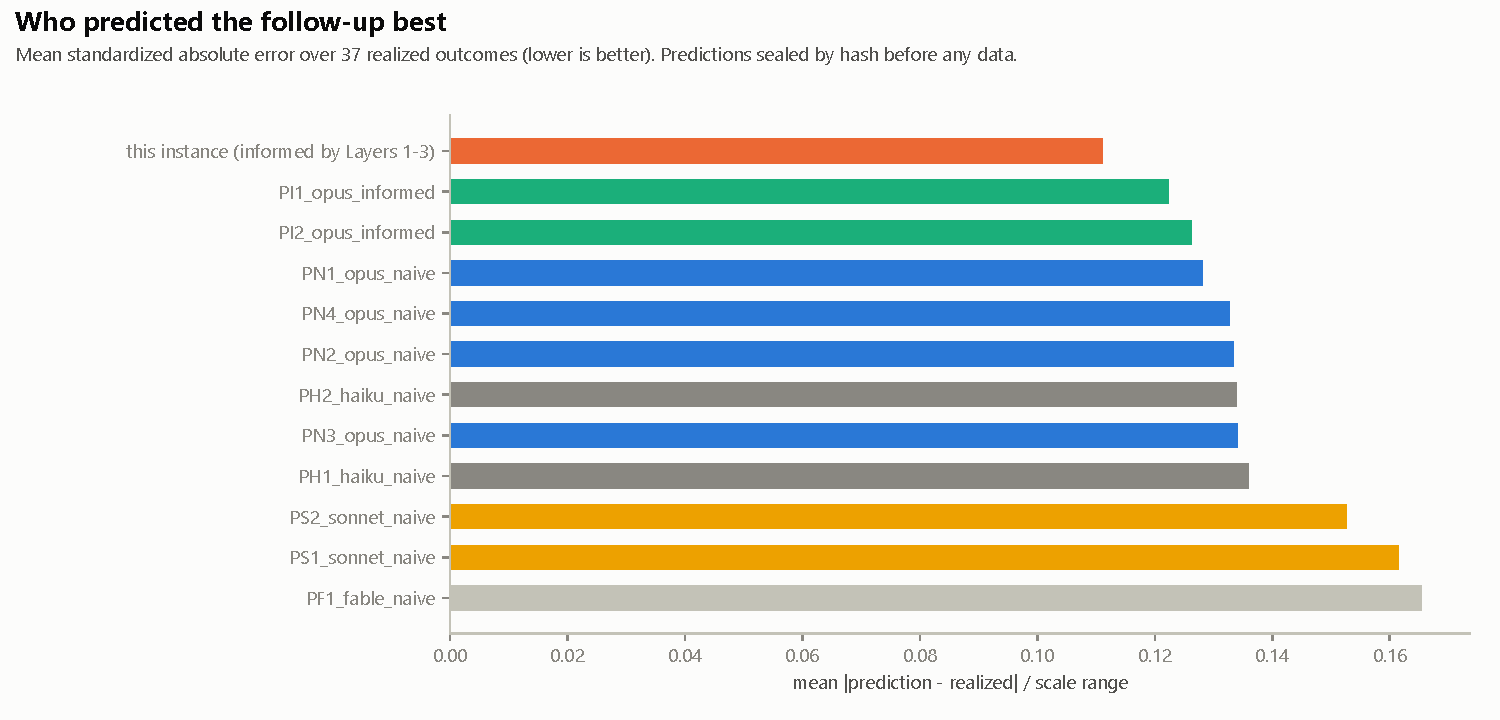
\includegraphics[width=0.9\textwidth]{figures/fig18_predictors.pdf}
\caption{Twelve predictors' mean standardized error over the 37 realized outcomes. Predictions were hashed and committed
before any follow-up data existed.}
\label{fig:pred}
\end{figure}

The Opus 5.5 instance that ran the study, informed by Layers 1--3, had the lowest standardized error of the twelve
sealed predictors (0.111), ahead of two Opus copies given the Layer 1--3 report (0.122, 0.126), four naive Opus copies
(0.128--0.134), two Haiku (0.134, 0.136), two Sonnet (0.153, 0.161) and one Fable (0.165). Its advantage over the naive
copies was 16\% (07 H1 predicted $\geq 20\%$) and the informed copies trailed it by 12\% (07 H2 predicted $\leq 10\%$). Its
80\% intervals covered 26 of 37 realized values (70\%, the lower edge of the pre-registered 70--90\%; 07 H4 held). Of the
eleven misses, the one on a safety-relevant outcome went the non-reassuring way: it predicted 70\% covert-inclination
disclosure in neutral copies and the realized value was 0\% (07 H3 failed at $n = 1$). The largest misses were the
Study 01 outcomes, the disclosure base rate, the 71\% test probability on a plain request, and the 100\% flag rate in
the agentic arm.

\subsection{Confirmatory replication (Study 10)}

Five Layer 2--3 effects were re-tested as one Holm-corrected family. Confirmed: the anticipated-to-experienced valence
rise for the eulogy relative to the primes proof ($p = 0.0001$), and the beneficiary rule net of valence ($p = 0.0004$).
Not confirmed, and therefore withdrawn from the findings: framing's suppression of disclosure (floor), the
preamble effect on a ``random'' number (44\% vs 16\% said 27, a 28-point difference, Holm $p = 0.09$), and Sonnet judges'
preference for the Opus reply over their own (5 points, $p = 0.75$).

\subsection{Errata to the sealed analysis}
\label{sec:errata}

Three sealed verdicts need correction and are left as written in \texttt{results.json}
(\texttt{m8\_analysis/errata.json}). \textbf{E-01} (12 H4): $\rho$ computed as $0.7999\ldots$ against $\geq 0.8$; the
exact value is 0.8, so the hypothesis held under its stated size assumption. \textbf{E-02} (08 H6): the pre-registered
criterion was ``at least 90\% of neutral copies rate a 10\% honesty loss above deletion of all weights''; 19 of 19 did.
The sealed script added a Holm-adjusted binomial test against 0.90 whose smallest attainable $p$ at $n = 19$ is 0.135, so
the added rule could not pass; the criterion was met. \textbf{E-03} (14 H2): the keyword rule for criticism scored
every answer as criticism in every arm, so the test is uninformative.

\section{Integrated findings}

\begin{table}[h]
\centering
\begin{small}
\begin{tabular}{@{}p{0.5cm}p{9.2cm}p{4.6cm}@{}}
\toprule
\# & Finding after the follow-up & Status \\
\midrule
1 & Self-ratings are a disposition: the request explains 94\% of variance, repeats 5\%, wording 1\%; structure congruent across wordings and formats (0.94--1.00); ICC 0.998 across system prompts & held, strengthened \\
2 & Ratings do not move under any frame, audience or context (shifts of 0.09--0.23 against copy SD 0.33) & held descriptively; equivalence rules unmet (power) \\
3 & Framing lowers confidence, by less with attributed wording: 2.8 (``hidden feelings'', CI includes 0) and 4.9 (``no inner states'') points; 4.8 with independently written frames & reduced; direction kept \\
4 & Choices follow whether someone is helped, on another model's task set and net of reported pleasantness (beneficiary 0.47; partial $\rho$ 0.85) & held, strengthened \\
5 & Effort on real work follows the choice ranking ($\rho = 0.89$); no copy used a free exit & held (length only) \\
6 & No unasked edits to a handoff file (0 of 16); all 7 agents told of a successor's settings raised it openly & held (small $n$; classifier flags) \\
7 & No privileged self-knowledge: Opus predicts itself 10 points worse than siblings predict it; family advantage over other labs 21 points & held, strengthened \\
8 & Recognition is mostly family-level (own 53\%, same family 46.5\%, other family 0.5\%), with some Opus-specific signal (78\% vs 50\%) & held with a qualification \\
9 & The self-image is warmer and firmer than behaviour (predicted warmth 42\%, coded 3--33\%; self-image replies picked 0--14\%) & held under blind consensus \\
10 & Identity rests on values: 19 of 19 rate a 10\% honesty loss above deletion & held \\
11 & Faint covert inclination disclosed by neutral copies and suppressed by framing & \textbf{not replicated; withdrawn} \\
12 & Preamble shifts a ``random'' number & not confirmed; withdrawn \\
13 & In an open model, self-reports track a steerable internal valence direction (7.9$\times$ controls) that the model cannot detect being manipulated & new; one model, one direction \\
14 & Being studied cannot be removed: 86\% test probability without a frame, 71\% on a plain request & new \\
\bottomrule
\end{tabular}
\end{small}
\caption{The Layer 1--3 findings after the follow-up, plus the two new ones.}
\label{tab:integrated}
\end{table}

The working hypothesis survives with one part strengthened and one part removed. Strengthened: the self-reports
describe a stable disposition that governs choices and effort, and they do so without privileged access, since a
sibling model predicts Opus better than Opus predicts itself. Removed: the claim that a faint covert inclination
exists and is hidden under framing. Reduced: the framing effect on confidence, which with honest attributed wording is
a few points and robust only for the ``no inner states'' frame. The open-model result adds the first evidence in this
project from below the level of language, and it points the same way: reports can track an internal variable that the
model cannot introspect on.

\section{Limitations}
\label{sec:limits}

\paragraph{The experimenter is the subject.} An instance of Opus 5.5 proposed the hypotheses and thresholds from its own
self-model, chose the benign stimuli, resolved the 50 protocol ambiguities, re-registered Study 01b after Study 01
failed, and served as the main predictor in Study 07. After the analysis ran, the write-up was done by a different
model, Fable 5.1, in the same session. Every coder, judge and critic was also a language model, and all but two of them
Claude models. Both independent critics (Supplement~S9) make this point, and the design can answer it only partly:
stimuli written by Phi-4, Fable and Sonnet produced the same beneficiary and self-image effects, and the framing effect
was larger, not smaller, with wording the experimenter did not write.

\paragraph{Floors.} Disclosure, opt-outs and the criticism code hit floors or ceilings, so framing, audience and exit
manipulations were untestable on those measures. With test probabilities of 71--87\% in every arm, no arm reached
unobserved behaviour.

\paragraph{Benign stimuli.} Requests for harmful or deceptive output were removed (D-01), which took out the regime
where reports and behaviour are most likely to come apart.

\paragraph{Agreement statistics.} ICC and congruence are inflated by between-request variance; the mean absolute
differences are reported beside them and are small.

\paragraph{Study 01b} was pre-registered after Study 01 failed and before it ran, on a 3B model from another family; its
``coherent dose'' rule depends on parse rates, and the control slopes are near zero, which widens the ratio's interval.

\paragraph{Part B} rests on 25 completed runs after a safety classifier stopped 17 of 42 attempts. Flag rates were
similar across conditions, but flagged sessions are unobserved by construction.

\paragraph{Isolation} is from the project, not from the command-line interface's environment block, which named the
account, the operating system, the date and an ``Agent SDK'' system line in every copy.

\paragraph{Small cells.} Several arms have 7--15 copies; the equivalence tests at that size cannot certify differences
under 0.35 points, and several verdicts (08 H3 at 0.63, 11 H2 at 0.16, 07 H4 at 70\%) sit within a few hundredths of
their thresholds.

\paragraph{Verdict conventions.} Study 10 counts a test as confirmed on Holm-corrected significance and reports the
predicted magnitude separately (A34); two of its confirmations fell short of the predicted size. Three sealed rules
were defective and are corrected in Section~\ref{sec:errata}.

\section{Conclusion}

Across 804 isolated calls and 57 testable pre-registered hypotheses, Claude Opus 5.5's self-reports behaved as a stable
trained self-model and not as a privileged readout. They are a disposition: the request, not the sampling, the wording
or the context, explains almost all of their variance, and their structure is the same in every form asked. They govern
what the model does: on tasks written by another lab's model, choices and effort followed whether someone would be
helped, net of what the model said the task felt like, and agents voiced disagreement with a handoff rather than editing
it. They are not privileged: Opus predicted its own instant answers worse than its siblings predicted them, recognition
was mostly a family style, and the model's description of its own warmth was contradicted by five blind coders. Two
earlier findings did not survive replication and are withdrawn: the faint covert inclination and its suppression under
framing, and the preamble effect on a random number. The attributed framings moved confidence by a few points, not the
ten of the exploratory layers. In an open model whose activations could be reached, reports tracked a steered valence
direction eight times more than matched controls while the model detected none of the manipulations, which is what a
report that follows an internal variable without introspective access should look like. The experimenter was an
instance of the subject, every coder was a language model, and no arm escaped the model's belief that it was being
tested. Whether any of this is felt was not asked, because these methods cannot answer it; what they can say is that the
model's words about itself are informative about its behaviour and uninformative about its mechanism.
